\documentclass[11pt]{article}
\usepackage[utf8]{inputenc}
\usepackage{graphicx}
\usepackage[ngerman]{babel}
\usepackage{url}
\usepackage{float}
\usepackage[backend=bibtex,style=alphabetic,sorting=ynt]{biblatex}
\usepackage[dvipsnames]{xcolor}
\addbibresource{literatur.bib}
\graphicspath{ {./images/} }
\title{
{Erstellung und Validierung eines Leitfadens zur Migration einer Microservice-Architektur nach Function as a Service}\\
{\large Frankfurt University of Applied Sciences}\\
}
\author{Gianni Pasqual}
\date{18.03.2020}
\begin{document}
\maketitle
\newpage
{\Large \textbf {Abstract}}
\\\\
Mit der Technologie Function as a Service ist nach der Microservice-Architektur eine noch feinere Modularisierungsstufe von Software erreicht worden. Mit dieser ist es möglich Software noch schneller bereitzustellen und im gleichen Zuge Einsparungen bei dem Betrieb der IT-Infrastruktur zu erzeielen. Dies erscheint auf den ersten Blick natürlich sehr lokrativ für viele Unternehmen, jedoch sollte die Entscheidung für den teilweisen oder gesamten Umzug der Service-Landschaft wohl überlegt sein. Wie bei jeder anderen Technologie hat auch diese ihre Potentiale und Herausforderungen die gemeistert werden müssen. Für Unternehemn, die sich dazu entschieden haben Function as a Service (FaaS) in ihre Infrastruktur einzubinden, soll diese Arbeit als Orientierung bei der Migration dienen. Da viele Unternehmen bereits von den monolithischen Anwendungen auf kleinere modularere Services umgestiegen sind, geht diese Arbeit von einer bereits vorliegenden Microserive-Architektur aus. Es gilt herauszufinden in welchem Maße und ob überhaupt strukturelle Anpassungen vorgenommen werden müssen, als auch der Frage nach "Best-Practices", nach nun knapp vier Jahren des Bestehens, nachzugehen.
\\\\
Zudem soll sich vor allem mit dem von den verschiedenen Anbietern ausgehenden Vendor-Lock-In auseinadner gesetzt werden und erarbeitet werden, welche Möglichkeiten bestehen, diesen zu umgehen bzw. zu mildern. Um mögliche Schwächen des Leitfadens aufzuzeigen, soll dieser beispielhaft an einem Service erprobt werden und auftretenden Fehler dokumentiert und behandelt werden.
\newpage
{\Large \textbf {Abkürzungsverzeichnis}}
\\\\\\
\begin{tabular}{ p{2cm} p{10cm}} 
 FaaS & Function as a Service \\ 
 IaaS & Infrastructure as a Service \\
 PaaS & Platform as a Service \\
 BaaS & Backend as a Service \\
 CaaS & Container as a Service \\  
 DevOps & Development and Operations \\  
 CI & Continuous Integration \\
 CD & Continuous Delivery \\  
 IT & Information Technology \\
 BDD & Behaviour Driven Development \\
 SDK & Software Development Kit \\
 DEV & Development \\
 VCS & Version Controle System \\
 INT & Integration (Testing) \\
 PROD & Production \\
 UAT & User-Acceptance (Testing) \\
 NIST & National Institute of Standards and Technology\\
 AWS & Amazon Web Services \\
 CNCF & Cloud Native Computing Foundatino \\
 XaaS & Anything as a Service \\
 RPC & Remote Procedure Call \\
 
\end{tabular}
\newpage
\tableofcontents
\newpage
\section{Einleitung}
\subsection{Forschungsfrage und Ziele der Arbeit}
\subsection{Erläuterung der Problemstellung}
\subsection{Aufbau der Thesis}










\section{Aufarbeitung des Themengebietes}
Ist eine Technologie, wie Function as a Service, noch relativ jung, so sind die Schritte der Findung einer in sich schlüssigen und allgemein vertretenen Definition oftmals noch nicht abgeschlossen. Auch bei der Definition von FaaS, Serverless und der Einordung dieser beiden Konzepte in die Infrastruktur des Cloud Computings8  \cite{mell2011nist}, ist dieser Prozess noch im Gange, wobei mitlerweile die unterschiedlichen Definitionen der offentlichen FaaS- und Serverless-Anbieter einige Gemeinsamkeiten aufweisen. Trotz alledem bestehen weiterhin ungenauigkeiten, die es in den nächsten Jahren noch zu beseitigen gilt. Hierzu später mehr. \\\\


\subsection{Definition des Begriffes Cloud Computing}
Der Begriff Cloud Computing ist laut eines Technology Report bis auf das Jahr 1996 zurückzuführen, wo er in einem Business-Plan des Unternehmens Compaq von ein paar Entwicklern genutzt worden sein sollen, um über die zukünftigen Entwicklungen des Internet-Businesses zu diskutieren \cite{regalado2011coined}. \\\\
Auch wenn das Konzept des Cloud-Computings, die dynamische, skalierbare, zuverlässige und unbegrenzte Bereitstellung von Ressourcen als Dienst über das Internet, immer mal wieder in der Literatur auftauchte \cite{fox2009above}, so erlangte es erst ab 2006 einen immer größter werdenden Bekanntheitsgrad. 2006 veröffentlichte AWS das Produkt Elastic Compute Cloud (EC2), gefolgt von Goolges App Engine 2008. Bereits in diesem früher Stadium wurde mit App Engine das Prinzip einer sog. \glqq stateful\grqq{}-Ebene, für das Speichern von des Aktuellen Anwendungsstatus und einer \glqq stateless\grqq{}-Ebene für die Ausführung des eigentlichen Programmes unterschieden \cite{fox2009above}. Des Weiteren wurde 2009 in einer Berkeley-Studie die sechs größten Potentiale des Cloud-Computings herausgearbeitet welche bis heute in den unterscheidlichen XaaS-Konzepten umgesetzt wurden. Im folgenden sind diese kurz auf gelistet. \\
\begin{itemize}
\item[1.] Unbegrenzte Ressourcen wann immer sie benötgt werden. 
\item[2.] Durch die Möglichkeit mit wenigen Ressourcen zu starten, vielen Nutzern zugang zu der Plattform zu gewähren. 
\item[3.] Die genutzen Ressourcen so genau wie möglich nach dem \glqq Pay Per Use\grqq{}-Prinzip zu bezahlen. 
\item[4.] Größenvorteile (Economies of scale) nutzen, um die Kosten durch eine dauerhafte, optimale Ausnutzung riesiger Datencenter auf ein Minimum zu reduzieren. 
\item[5.] Operationelle Kosten so weit es geht zu senken und die Ressourcennutzung durch Virtualisierung so weit wie möglich auszunutzen. 
\item[6.] Eine hohe Hardwareausnutzung durch \glqq Multiplexing\grqq{} der Auslastungen verschiedener Unternehmen zu erreichen.
\end{itemize}
Das National Institute of Standards and Technology (NIST) veröffentlichte 2011, nach 16 vorausgehenden Definitionen, schließlich eine finale Definition des Cloud-Computings, welche bis heute als orientierung Anwendung findet und in einer vielzahl an Werken aufgegriffen wird \cite{mell2011nist}. Die Definition nach NIST beschreibt das Cloud model als eines aus fünf essentiellen Charakteristiken und drei Service Modellen, IaaS, PaaS und SaaS bestehendes Modell, mit insgesamt vier Deployment-Models. \\\\
\textit{"Cloud Computing is a model for enabling ubiquitous, convenient, on-demand network access to a shared pool of configurable computing resources (e.g., networks, servers, storage, applications, and services) that can be rapidly provisioned and released with minimal management effort or service provider interaction."} \cite{mell2011nist}.\\\\
NIST bricht die Definition mit Essentiellen Charakteristiken, Service-Models und Deployment-Models in drei Unterkategorien herunter, welche erfüllt sein müssen um dem Anspruch an Cloud Computing zu genügen. \\
Grob gefasst sind dies bei den Characteristiken, die automatische Bereitstellung der benötigten Ressourcen je nach bedarf (\textit{On-demand self-service}), die Möglichkeit von allen gängigen Geräten darauf zugreifen zu können (\textit{Broad network access}), die optimale Verteilung von Ressourcen auf die Kunden welche sie gerade benötigen, wobei hier die exakte lokation dieser von geringer Relevanz ist (\textit{Resource pooling}), die automatische Skalierung von Ressourcen (\textit{Rapid elasticity}) und die Möglichkeit der Überwachung und Limitierung der Ressourcenausnutzung, welche für den Kunden als auch den Anbieter transparent sein muss (\textit{Measured service}).\\\\
Bei den Service Models werden hier lediglich IaaS, PaaS und SaaS unterschieden. Laut NIST gibt es um den Code in der Could bereitzustellen vier verschiedene Deployment-Models, welche genutzt werden können. Mit der \textit{Private cloud}, obliegt es dem Unternehmen seine Infrastruktur komplett selber zu betreiben, jedoch muss diese dem Unternehmen dabei nicht selber gehören, sondern kann von eine dritten Partei gehostet werden. Mit dem deployment auf eine \textit{Community cloud} teilen sich verschiedene Unternehemen eine Cloud, welche entweder von ihnen gemeinsm, oder von einem Drittanbieter betrieben wird. Zuletzt gibt es noch die Möglichkeit die von einem Cloud-Computing-Anbieter bereitgestellte öffentliche Cloud \textit{Public cloud} zu nutzen, bei welcher das Unternhemen die Räumlichkeiten bzw. Ressourcen von einem Dittanbieter nutzt. Das letzt Deployment-Model stellt die sog. \textit{Hybird cloud} dar, welche eine Kombination aus den vorherigen darstellt \cite{mell2011nist}.
\begin{figure}[H]
\caption{Übersicht Service-Models Cloud-Computing}
\label{fig:cloudComputingConcepts}
\centering
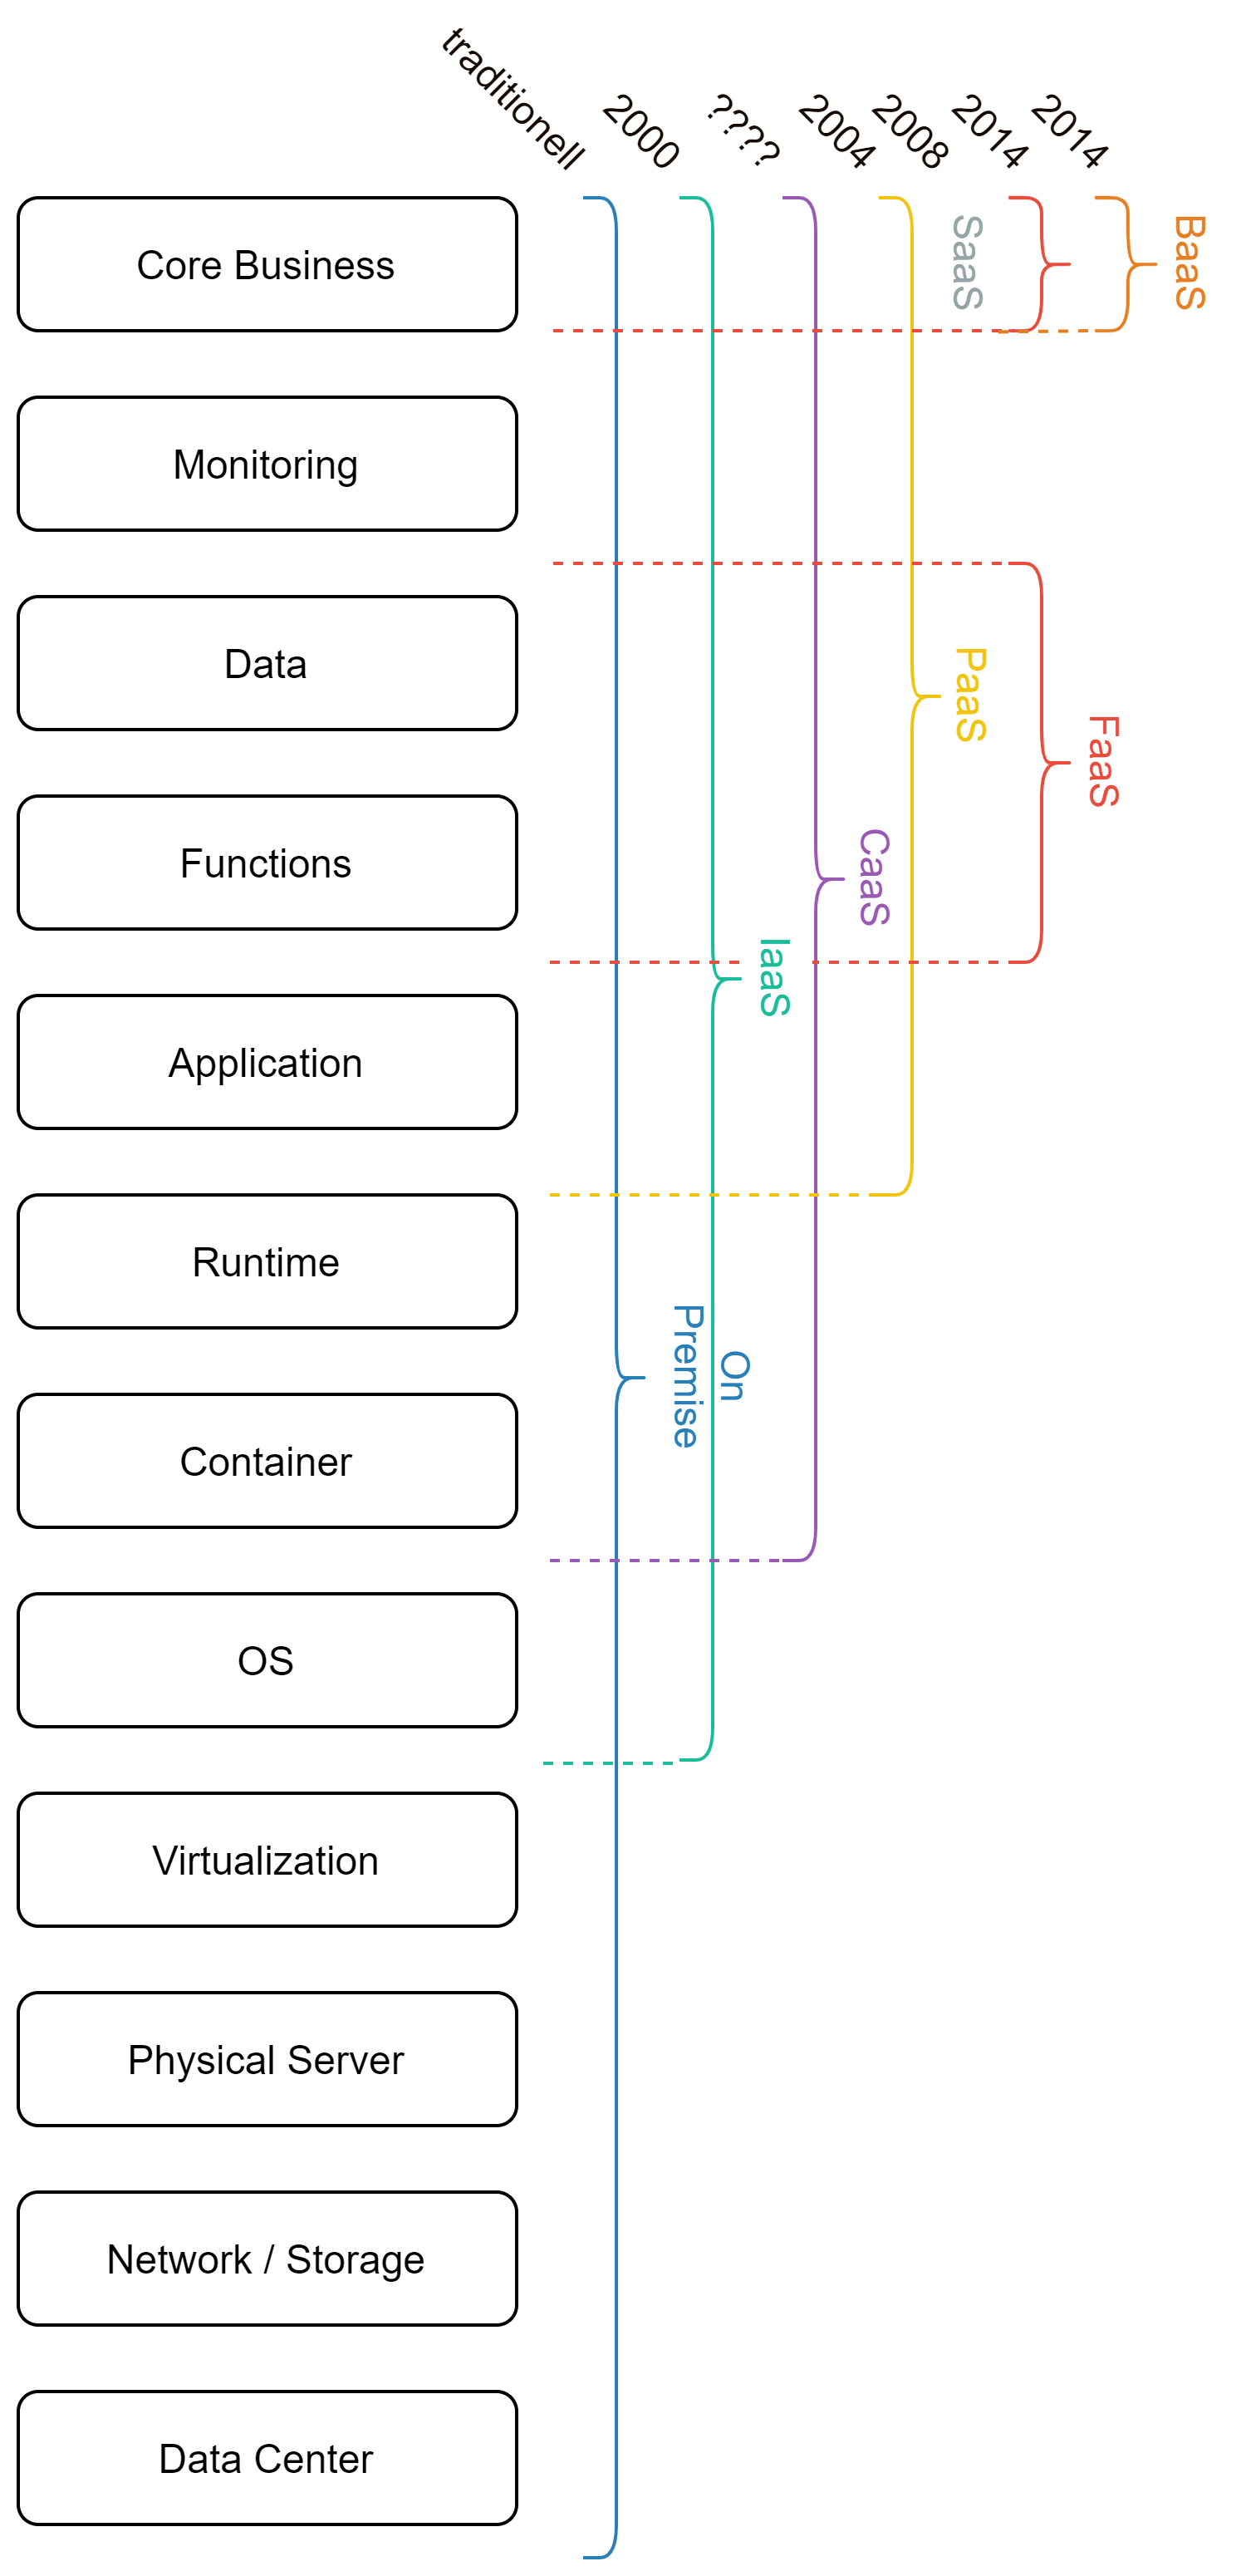
\includegraphics[angle=90,width=1\textwidth]{serviceModels}
\end{figure}
Neben den bereits genannten Service Models IaaS, PaaS und SaaS gibt es jedoch noch weitere, welche sich im Laufe der Zeit etabliert haben. Abbildung ~\ref{fig:cloudComputingConcepts} gibt einen Überblick hierüber. 


\subsection{Function as a Service}
Function as a Service (FaaS) ist ein sogenanntes \glqq Serverless\grqq{} Cloud-Computing Konzept, welches erstmals 2014 von AWS mit Lambda Functions als Preview Release und schließlich 2015 zur kommerziellen Nutzung zur Verfügung gestellt wurde \cite{aws2020LambdaFunctions}. Es kann nach IaaS und PaaS als ein weiterer Schritt in der Entwicklung des Cloud Computings gesehen werden, welcher das Management von Infrastruktur, Servern und Ressourcen weg von dem Entwickler nimmt und hin zu dem Cloud-Anbieter delegiert. Ein knappes Jahr später, 2016, traten Microsoft mit Azure Functions, Google mit Google Cloud Functions und IBM mit OpenWhisk in den bis dahin von Amazon dominierten Markt ein. Mittlerweile gibt es eine vielzahl an Open-Source sowie proprietären Anbietern, welche um die Gunst der Kunden werben und einen stetigen Wettbewerb aufrecht erhalten. Ein ausführliche Übersicht über die jeweiligen Anbiter findet sich online von der CNCF \cite{cncf2020ServerlessLandscape}\\\\
Da es sich mit FaaS und Serverless um eine noch recht junge Technologie handelt gibt es zu diesem Konzept keine offiziell dokumentierte Definition. bsp. von NIST o.ä., in der Literatur, wie es beispielsweise beim Cloud-Computing \cite{mell2011nist} der Fall ist. Die Anbieter sind sich jedoch über die Funkitionalität von FaaS größtenteils einig, was das Spektrum an Funktionalitäten anbegeht. So definiert Microsoft Azure Functions als: \glqq [...] event-driven serverless compute platform that can also solve complex orchestration problems. Build and debug locally without additional setup, deploy and operate at scale in the cloud, and integrate services using triggers and bindings. \grqq{} \cite{azure2020Functions}. Hiermit beschreibt der Anbieter bereits die Kernfunktionalitäten von FaaS und drückt den Kerngedanken hinder FaaS aus. Das Konzept soll genutzt werden können, um bei dem Auftreten eines zuvor definierten sog. Triggers auf ein Event aus der eigenen Applikation oder der des Abieters reagieren zu können. Dabei stellen die meisten Anbieter wie Google, Azure oder AWS neben einem einfachen event-basierten HTTP-Trigger oder widerkehrenden zeitbasierten Triggern noch weitere, an die jeweilige Infrasturktur des Anbieters angepasste, Trigger zur Verfügung. Diese ergeben sich meist aus den BaaS Angeboten, hierzu mehr in \textit{Abgrenzung von FaaS zu Serverless}, welche in Form von Datenbank Triggern bei einer CRUD-Operation, dem Anlegen eines Nutzers oder der Integration mit einem Push-Notification Service [AWS SSN, Google Pub/Sub etc.] auftreten können.\\
\begin{figure}[H]
\caption{FaaS Programming Model nach OpenWhisk \cite{openWhisk2020ProgrammingModel}}
\label{fig:openWhiskProgrammingModel}
\centering
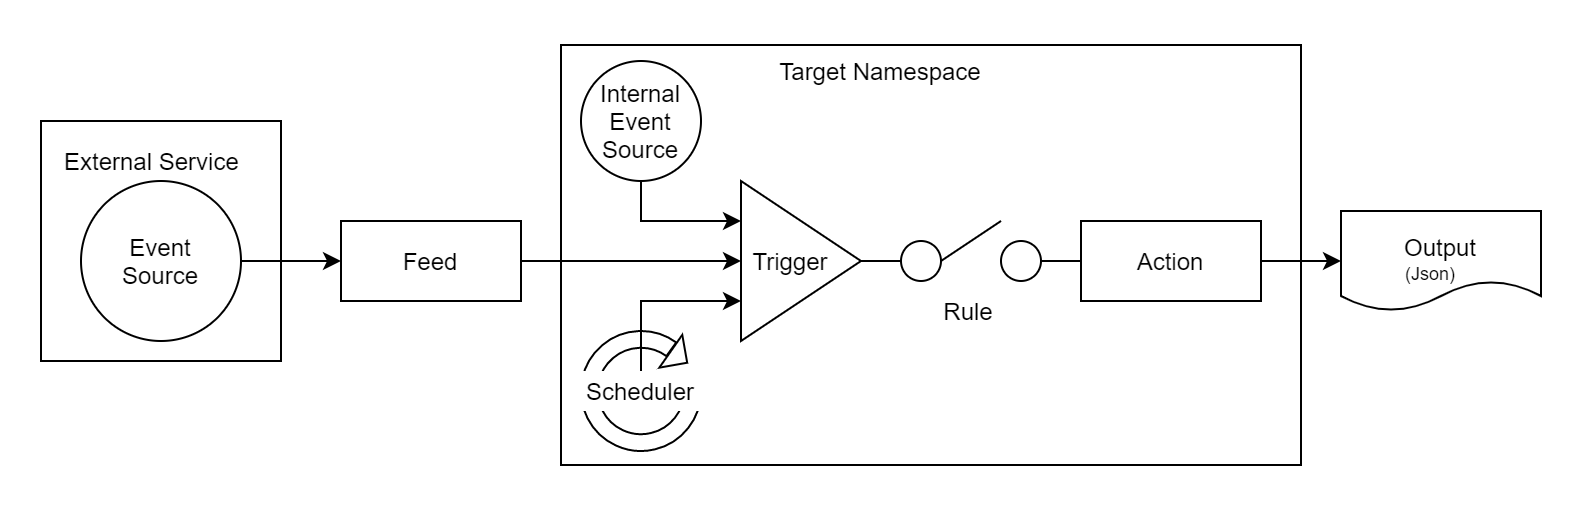
\includegraphics[width=1\textwidth]{ProgrammingModel}
\end{figure}
Abbildung ~\ref{fig:openWhiskProgrammingModel} gibt hierbei eine Übersicht über die verscheidenen Event-Trigger, welche derzeit bei den großen, proprietären Anbietern (AWS, Google, Microsoft) existieren. Da hinter OpenWhisk mit IBM eine großes Unternehmen steht, wird dieses Modell in der Literatur häufig als Referenz in Bezug auf die anderen Anbieter verwendet. Es kann angenommen werden, dass andere Abieter ein ähnliches Konzept bei ihrer FaaS Architektur verfolgen, da Apache OpenWhisk in einer großen Cloud (IBM) bereitgestellt wird \cite{van2019spec}. Eine weitere fundamentale Eigenschaft ist die erwähnte Skalierbarkeit, welche nach dem sog. \glqq Pay Per Use\grqq{}-Modell abgerechnet wird. Gemeint ist hiermit, dass der Kunde nur das bezahlt was er auch wirklich verbraucht hat, wobei die Verrechnung extrem granular nach genutzten Ressourcen und gelaufener Zeit erfolgt. Der Kunde bezahlt daher nicht für die benötgten Ressourcen, wie er es bei PaaS (wobei es hier variierende und bereits granularere Modell gibt) oder IaaS der Fall ist, sondern nur für die tatsächlich genutzten Ressourcen. \\\\
\textcolor{blue}{Grundsätzlich ist zwar der Preis der für das Laufen einer einminütigen Funktionsaussführung verglichen mit dem Laufen des selben Codes auf einem von den Ressourcen her ähnlich bestückten PaaS-Server günstiger \cite{jonas2019cloud}, jedoch der Anwendungszweck ein ganz anderer. Während mit PaaS Anwendungen bedient werden, die eine dauerhaft hohe Nachfrage erfahren, sollen mit Funktionen primär einfache stark frequentierende Aufgaben geläst werden, bei denen der Nutzer nur für die Ressroucen bezahlen muss die die Funktion bei dem Aufruf nutzt und nicht für jene die ohen einkommende Aufrufe provisioniert wurden.} \\\\
Ein weiterer wichtiger Punkt, welcher sich auch bei anderen Anbietern findet, ist in der Definition von OpenWhisk zum einen mit \glqq[...] you can focus on building amazing and efficient applications [...]\grqq{} und zum anderen mit \glqq  developers write functional logic [...] in any supported programming language, that can be dynamically scheduled [...]\grqq{}\cite{apache2020OpenWhisk}. Ersteres meint die Abstraktion der Infrastruktur, welche dem Nutzer zum Bereitstellen von lauffähigem, skalierbaren, sicheren Backend-Code nicht bekannt sein muss. Die automatische Skalierung und optimale Verteilung von Ressourcen obliegt der Hoheit des Anbiters, und ist dem Nuzter nicht zugänglich, zumindest bei den proprietäre Anbietern. Letzteres ist zwar keine einzigartige Eigenschaft von FaaS, da dieses Konzept beriets lange bekannt ist und auch bei der Microservice-Enticklung häufig zum Einsatz kommt, jedoch ist die Auswahl aus vielen verschiedenen Programmiersprachen wie Java, Go, Javascript (Typescript), Python, PHP usw. (abhängig von dem jeweiligen Anbieter) unter dem Gesichtspunkt der direkten Nutzung zu sehen. Es muss keinerlei zusätzliches Setup oder andere Konfigurationen in der Umgebung vorgenommen werden, da dies der Anbieter übernimmt. Er kümmert sich um Patches und das Upgraden auf die aktuellste Version, was dem Entwickler ein großes Maß anflexibilität bei der Entwicklung der Anwendung einräumt. Eine weitere häufig in der Literatur referenzierte Defninition ist \cite{fowler2018serverless}, von Mike Roberts, welche die Beschreibung von AWS Lambda näher erläutert und im groben die oben genannten Punkte wiedergibt. \textcolor{blue}{Natürlich sind diese Eigenschaften mit einem gewissen Venodr Lock-In \textcolor{red}{dieser jedoch weder als schlecht noch gut zu bewerten ist und vielmehr nüchtern auf seine Vor- und Nachteile anasystiert werden sollte.} verbunden, da dieser Enstcheidungen über die Infrastruktur trifft, mehr dazu in \textit{Potentiale und Herausforderungen}.}\\\\
Abbildung ~\ref{fig:FaaSBaaSExample} verdeutlicht hierbei noch einmal die Wirkungsweise von FaaS. Oben rechts ist der Funktionspool zu sehen, welcher bei dem jeweiligen Cloud Provider steht und in welchen der Entwickler seine Funktionne lädt. Wird eine Funktion von einem Client aufgerufen, so wird bei Aktivierung eines Triggers eine Kopie der jeweiligen Funktion instantiiert und alle mit diese Funktion verbundenen Abhänigkeiten geladen (bspw. benötigte Module). Je nachdem wie frequentiert die Funktionen von den Clients angefordert werden, werden die vorhandenen Instanzen automatisch von dem Provider 
\begin{figure}[H]
\caption{Anwendung mit FaaS und (P)BaaS, angelehnt an \cite{shafiei2020serverless}}
\label{fig:FaaSBaaSExample}
\centering
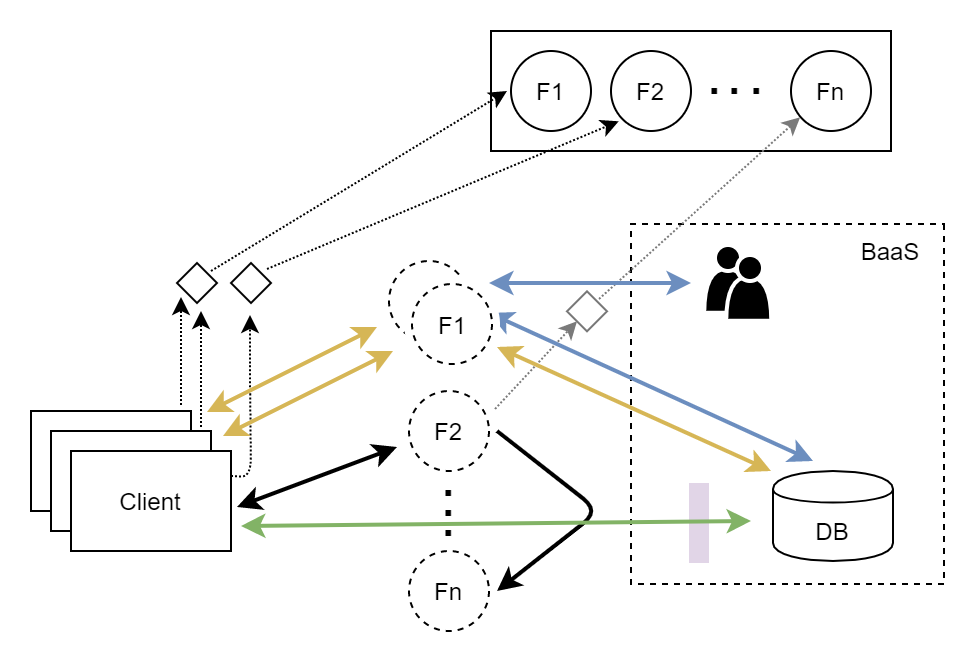
\includegraphics[width=1 \textwidth]{FaaS}
\end{figure}
hochskaliert, um den eingehenden Anfragen gerecht zu werden. Hierbei kann die Funktion eine Aufgabe direkt ausführen und das Resultat an den Client zurückgeben, oder wie bei F1 auf die im hintergrund laufende BaaS Infrasturktur zugreifen. Diese reicht von einfachen Datenbankabfragen bis hin zu anlegen eines neuen Nutzers etc. Limitiert werden die Möglichkeiten hierbei lediglich von dem Service-Ökosystem des jeweiligen Anbieters. Genauso ist es natürlich möglich Funktionen sich gegenseitig aufrufen zu lassen oder direkt mit BaaS-Servicen zu interagieren, siehe \textit{Abgrenzung von FaaS zu Serverless}. \\\\
Um FaaS besser und einheitlicher definieren zu könne und damit einen plattformübergreifenden Standart zu schaffen, wird in der Industrie und Forschung das Verlangen nach einer Referenzarchitektur, wie sie beispielsweies für das Cloud oder Grid Computing vorhanden ist \cite{liu2011nist}, \cite{foster2003grid} lauter. Die Abwesenheit einer solchen Architektur behindere die Etablierung von Best-Practices, Design Pattern und einen genaueren Überblick darüber zu erhalten, wie sich das Feld rund um Function as a Service entwickele \cite{leitner2019mixed}. Erste Vorschläge wie die Referenzarchitektur von FaaS aussehen könnte, haben sich mit \cite{van2019spec} durch die über die Jahre, von 2016 an, gestiegenen Popularität von Faas in der Forschung und der Literatur bereits herausgebildet. War hier die Thematik bis 2016 nicht addressiert worden, so stieg die Präsenz von hier an kontinuierlich bis 2019, in Journals, Konferenzen und Workshops an \cite{Yussupov2019_SystematicMappingStudyFaaS}. \\\\


\subsection{Abgrenzung von FaaS zu Serverless}
Serverless-Computing, oftmals auch als Serverless bezeichnet, ist eine Teildisziplin des Cloud-Computings, welche sich aus der Virtualisierung von Rechenleistung, Speicher und Netzwerken aus entwickelt hat \cite{jackson2018investigation}. Wie so häufig ist die Abgrenzung bzw. die Unterscheidung bei sich neu entwickelden Technologien nicht ganz einfach. Zunächst stand Serverless für Anwendungen welche teilweise oder komplett auf Drittanbieter zurückgriffen, auf sog. Backends as a Service (BaaS) [siehe Abbildung. ~\ref{fig:serverlessBaaSandPaas}], um serverseitige Aufgaben wie Datenbankabfragen, Nutzerverwaltung o.ä. zu regeln \cite{fowler2018serverless}. \\\\
Mit FaaS wurde das Serverless-Konzept dahingehend erweitert, dass die Serverlogik nicht mehr vollständig von einer dritten Partei zur Verfügung gestellt wird, sondern vom Entwickler selber implementiert werden kann. Serverless ist dabei eines der in den letzten Jahrne häufig genutzten Basswords in der IT, wobei der Begriff an sich etwas anderes suggeriert, als das was damit tatsächlich gemeint ist. Der Begriff impliziert die Abwesenheit von Servern, wobei damit lediglich eine Verschiebung der Zuständigkeiten einher geht. Entwickler einer \glqq Serverlosen\grqq{}-Anwendung bspw. mit FaaS, müssen sich nicht mit den operationellen Tätigkeiten wie dem \textit{Provisioning}, Monitoring, der Wartung der Infrastruktur, der Skalierbarkeit dieser und der Robustheit des Systems befassen \cite{baldini2017serverless}. Jedoch geht mit der Abgabe an Zuständigkeiten auch ein gewisser Vendor Lock-In einher, wobei die Anbeiter darauf achten, das mit FaaS eine möglichst große Zahl der in ihrem Service-Ökosystem vorhandene Services genutzt werden \cite{kritikos2018review}. Es sollen möglichst viele der bereits im vorherigen Abschnitt vorgestellten Trigger bei dem Bau von Anwendungen genutzt werden. \\\\
Function as a Service ist somit zum Großteil aus dem Event-Driven Computing, welches vor allem bei der UI-Entwicklung genutzt wird, abgeleitetes Konzept, welches Serverless-Computing adaptiert hat. Nichts desto trotz wird der Begriff Serverless in vielen Fällen, laut \cite{leitner2019mixed} in 58\% der Fälle, mit FaaS gleichgesetzt, was eine Abgrenzung erschwert. Abbildung ~\ref{fig:serverlessBaaSandPaas} verdeutlicht in welcher Beziehung die unterschiedlichen Konzepte stehen. 
\begin{figure}[H]
\caption{Serverless Concept, including FaaS and BaaS}
\label{fig:serverlessBaaSandPaas}
\centering
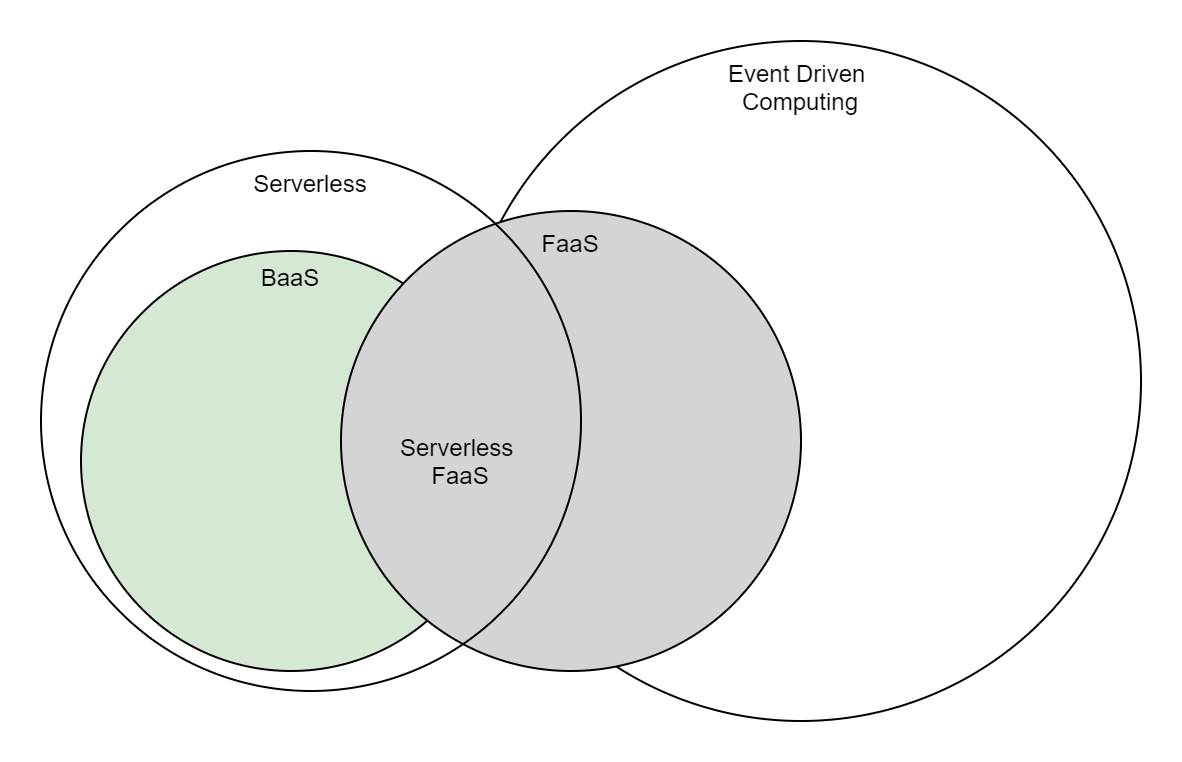
\includegraphics[width=1\textwidth]{Serverless}
\end{figure} 
Besteht eien Anwendung in der Folge lediglich aus den zwei \glqq serverlosen\grqq{} Komponenten, FaaS und BaaS, so ist häufig die Rede von einer \glqq pure serverless\grqq{}, also einer Anwendung, deren operationeller Teil vollständig an einen Cloud-Anbieter ausgelagert wurden und einer \glqq hybrid serverless\grqq{} Anwendung unterschieden \cite{leitner2019mixed}. Bei letzterem fungieren die Kunktionen häufig als sog. \glqq Glue\grqq{}, der meisten zeitlich variierend Aufgaben übernimmt, da IDLE-Zeit, wie man sie aus IaaS oder PaaS kennt, nicht berechnet wird.\\\\Nun mag der ein oder andere argumentiern, das ein Großteil der infrasturkurellen Aufgaben auch bei PaaS von dem Cloud-Anbieter übernommen werden, womit er natürlich recht hat. FaaS geht an dieser Stelle jedoch noch einen Schritt weiter. Bei Paas werden vorgefertigte \textit{Packages} einer Anwendung auf der Runtime der entsprechenden Plattfrom bereitgestellt, womit sich die Entwickler immer noch im die Anwenungsstruktur kümmern müssen \cite{kaplan2019framework}. In FaaS hingegen wird dieser Teil übernommen und der Entwickler konzetriert sich lediglich auf die Business logik und die jeweiligen Event-\textit{Trigger}. \\\\
Zuletzt soll noch auf einen weiteren Punkt, \glqq NoOps\grqq{}, eingegangen werden, der oft mit Serverless gleichgestellt wird. Es wird zwar durch die Übernahme des Loadbalancing, der automatischen Skalierung, Sicherheitsaspekten und Patches ein Großteil der Wartung ausgelagert, jedoch ist dies nicht mit der Annahme des Wegfalls der Operations von DevOps gleichzusetzten, wie suggeriert wird \cite{fowler2018serverless}. Es obliegt weiterhin den Entwicklern qualitativ hochwertigen Code zu schrieben und diesen in der Cloud-Umgebung zu testen, um dessen Performanz sicherzustellen. Die Komplexität entfällt daher nicht vollkommen, sondern verlagert sich zu einem gewiessen Teil \cite{eivy2017wary}. \textcolor{red}{Schaut man sich beispielsweise AWS an, so muss eine vielzahl an Konfigurationen vorgenommen werden. Zwar kann später eine vorhanden auf alle Funktionen angewendet werden, jedoch ist diese in der Folge von essentieller Bedeutung in einer riesigen \glqq Multitennacy\grqq{}-Umgebung.}\\\\% however, developers of serverless applications do not have to deal with any operational management with respect to provisioning, monitoring, maintenance,scalabilityandresilienceoftheserverstheapplicationisdeployedon \cite{baldini2017serverless}


\subsection{Potentiale und Herausforderungen}
Die im Folgenden aufgelisten Potential und Herausforderungen, denen sich Literatur und Anwender von FaaS gegenübersehen, sind zu Teilen dem Konzept selber, zu Teilen aber auch der Implementation der jeweiligen Anbeiter bzw. Open-Source Lösungen geschuldet. Es werden daher auf Seiten der Herausforderungen diese zunächst erläutert und falls in der Literatur bereits adressiert, vorgeschlagen Lösungen aufgezählt. Bei beiden, Potentiale und Herausforderungen, wird sowol Bezug auf FaaS als auch auf BaaS genommen, da diese beieden Kategorien in den meisten Fällen in Kombination genutzt werden bzw. architektionisch beding in Kombination genutz werden müssen [siehe Abbildung ~\ref{fig:serverlessBaaSandPaas} und \glqq statelessness\grqq{} Abschnitt \textit{Function as a Service}]. \\\\\\
{\normalsize \textbf{Potentiale}} \\\\
\textbf{Kosteneffizienz}\\
\\\\
\textbf{Time to Market / Lead Time Development}\\
\\\\
\textbf{DevOps}\\
\\\\
\textbf{Testing}\\
\\\\
\textbf{Optimale Auslastung von Rechenzentren}
Greener Computing \cite{shafiei2020serverless} \cite{fowler2018serverless}
\\\\
{\normalsize \textbf{Herausforderungen}} \\\\
\textbf{Vendor Lock-In}
Auch wenn diese Eigenschaft sowohl 
\textbf{Physische Lokation}\\
Eine weiterer Punkt ist die physische Lokation der Funktionen. Dadurch, dass es dem Provider obliegt, die Ressourcen seiner Infrastruktur optimal zu nutzen, entscheidet dieser auch auf welcher Node eine Funktion ausgeführt wird. Platziert der Provider in der Folge Funktionen, die eine hohe Datenabhänigkeit haben, physische weit voneinander entfernt, so wird sich dies auf die Performance der Anwendung auswirken und letztlich als Latenz bei dem Endverbraucher zu spüren sein \cite{shafiei2020serverless}. Es gibt zwar bereits bei vielen Anbietern, wie AWS, Microsoft oder Google die Möglichkeit die Region beziehungsweise ein sog. Cluster festzulegen, jedoch lässt sich damit die Lokation lediglich eingrenzen, aber nicht rechenzentren-genau festlegen. Mit der Performance von \glqq serverful\grqq{}-Applikationen kann damit nicht gleichgezogen werden \cite{shafiei2020serverless}. \\\\
\glqq \textbf{Serverless}\grqq{}\\
Es ist an dieser Stelle zwar relativ trivial, trotz alledem ein Nachteil verglichen mit Lösungen wie PaaS oder IaaS. Die Rede ist von dem Verlust der serverseitigen Optimierung. Wie bereits durch den Namen deutlich gemacht, existieren die Server für den Nutzer nicht bzw. hat er bei einer auf BaaS basierenden Softwarelösung keine Kontrolle über das Backend. Er kann lediglich die Datenbanken, Objektspeicher oder Authentifizierung an die Struktur seiner Daten anpassen und über \glqq Regeln\grqq{}Zugriffsbeschränkugen umsetzen. Die Services sind von dem jeweiligen Vendor vorgegeben und können bspw. nicht nach dem \glqq Backend For Frontend\grqq{}-Muster \cite{sam2015bff} auf die entprechenden Client-Typen, wie Tablet, Mobile-Phone oder Desktop angepasst werden. Es existieren von jeder Sorte (Datenbanken, Objektspeicher, Authentifizierung usw.) nur eine Version auf welche man beschränkt ist. Jegliche benutzerdefinierte Logik muss daher in den Client ausgelagert werden, da es nicht auf backendseitig implementiert werden kann \cite{fowler2018serverless}. Mit FaaS kann dieser Effekt gemindert werden, indem ein leichtgewichtige Logik in form von Funktionen serverseitig umgesetzt wird. Hierbei erfolg die Interaktion mit den unterschielichen BaaS-Servicen über die vom Anbieter beschränkten Trigger [siehe Abschnitt \textit{Function as a Service}]. \\\\
\glqq \textbf{Statelessness}\grqq{}\\
Mit der \glqq statelessness\grqq{}, also der Zustandslosigkeit von Funktionen, geht eine weitere Problematik von FaaS einher. Der Kern von Anwendungen ist es Aufgaben zu lösen, wofür viele verschiedene Schritte von Nöten sind, welche sinnvoll miteinander verbunden werden müssen. So ist es auch bei dem funktionsbasierten Aufbau von Applikationen wichtig, dass diese untereinander kommunizieren können und den Programmstatus voneinander abfragen können, ohne das es zu Inkonsistenzen kommt. Bedingt durch die kurze Laufzeit der Funktionen ist es essentiell, dass auch der Austausch in entsprechender Geschwindigkeit erfolgt. Wie in einem Report von Berkeley \cite{jonas2019cloud} herausgearbeitet, erweist sich das schnelles und exaktes \glqq State-Sharing\grqq{} jedoch immer noch als problematisch dar, betrachtet man die Geschwindigkeit von \glqq Serverless\grqq{}-Anwendungen im Vergleich mit \glqq Serverful\grqq{}-Anwendungen. \\\\
Grund hierfür sind die von den Anbietern zur Verfügung gestellten BaaS-Lösungen für das persistente Speichern des Programmstatus. Objektspeicher der verschiedenen Anbieter (AWS S3, Google Cloud Storage, Azure Blob Storage) sind zwar nicht teuter sehr teuter wenn es um das Speichern mehrerer GB geht, jedoch sind die Kosten beim Zugreifen auf die Speicher hoch und die Latenzzeiten von bis zu 20ms zu hoch \cite{jonas2019cloud}. Die Key-Value-Speicher der Anbieter sind in diesem Falle die bessere Wahl, da ihre Ansprechzeiten mit 8 - 15ms geringer sind, jedoch sind sie, bezogen auf ihre Input/Output Operationen pro Sekunde, deutlich teurer als die der Objektspeicher. \\\\
Neben dem schnellen Informaitonsaustausch der Funktionen mit einem externen Speichermedium, kann es bei einer Kopplung von Funktionen aus performancetechnischen Gründen sinnvoller sein, den aktuellen Programmstatus direkt and die nächst Funktion weiter zu geben. Wie zuvor bei der \textit{physischen Lokation} der Funktionen erwähnt, ist es wahrscheinlich, dass Funktionen nicht auf der selben Node gestartet werden. Der Loadbalancer des jeweiligen Providers entscheidet je nach Auslastung der Infrasturktur, auf welcher Node eine Kopie der Funktion ausgeführt wird. Auch wenn im Idealfall die Weitergabe des \glqq application states\grqq{} schneller ist als der Zugriff auf ein externes Speichermedium, so wird dies durch \glqq Startup-Latencies\grqq{}und physischer Distanz wieder relativiert. Um dem entgegenzuwirken schlagen Shafiei et. al. \cite{shafiei2020serverless} vor, mit einem \textit{Dependency-Graphen} miteinander verwobene Funktionen zu kennzeichnen und direkt bei dem initialen Aufruf einer Funktion mögliche Folgefunktionen zu starten. \\\\
Würde man dem Nutzer die Möglichkeit geben zu bestimmen auf welcher Instanz (Node) eine Funktion laufen soll, so das Konzept von FaaS damit untergraben werden (siehe \textit{Optimale Auslastung}). Es würde dazu führen, dass erneut Kapazität zurückgehalten wird, über welche der Provider nicht mehr frei verfügen könnte. 
\begin{figure}[H]
\caption{Dependency Graph nach \cite{shafiei2020serverless}}
\label{fig:dependencyGraph}
\centering
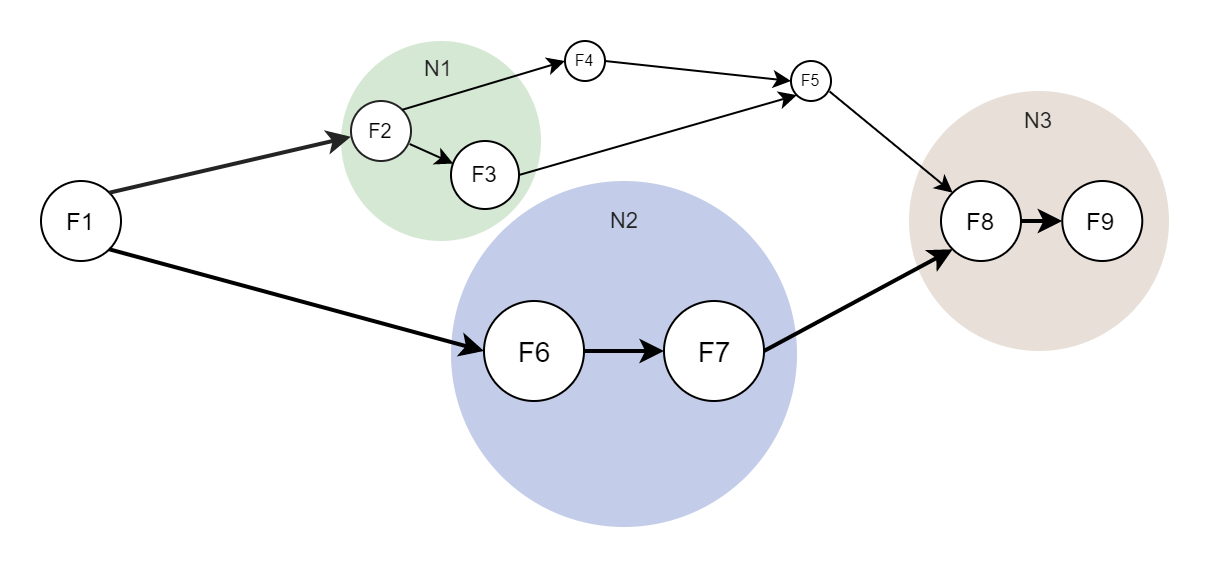
\includegraphics[width=1\textwidth]{DependencyGraph}
\end{figure} 
Wenn jeder Nuter bestimmen könnten auf welcher Node, bspw. Node-X, seine Funktionen laufen sollen, um den Progrmamstatus mit so wenig physisch bedingter Latenz wie möglich weiterzugeben, so wäre eine optimale Auslastung nicht mehr garantiert. Der Provider müsste stets Kapazität von Node-X zurückhalten und könnte sie nicht für andere Nutzerfunkitonen freigeben. Er muss stets einen Teil der Kapazität von Node-X zurückhalten, für den fall dass inaktive, aber der Node zugeteilte Funktionen aufgerufen werden. Mit einem \textit{Dependency-Graphen} wie in Abbildung ~\ref{fig:dependencyGraph} zu sehen würde dieses Problem umgangen werden. Der \textit{Load-Balancer} des Anbieters könnte unbeinträchtigt die Funktionen wie gewohnt je nach Auslastung auf freie Nodes verteilen, da er die korrelierenden Funktionen \glqq gleichzeitig\grqq{} starten kann. Da die Latenzen beim Starten eines Services erheblich höher sind, wobei die Programmiersprache dies zusätzlich beinflussen kann \cite{manner2018cold}, als jene durch die Lokation bedingt \cite{aditya2019will} \cite{jackson2018investigation}, würde deren Eliminierung die Weitergabe des \textit{States} erheblich beschleunigen. \\\\
Generell betrachtet könnte die Geschwindigkeit der Kommunikation von Funktionen untereinander beschleunigt werden. Verbindet man das ganze noch mit einem einfachen neuronalen Netz, um beispielsweies vorherzusagen mit welcher Wahrscheinlichkeit Funktion zwei (F2) im Vergleich zu Funktion sechs (F6) angesprochen wird, so könnte die Performance sogar noch ressourcenschonender auf Seiten des Cloud-Providers gestaltet werden. Zunächst käme es entweder zu einer höhreren Belastung, sollte man zu Beginne alle Funktionen starten oder zu einer höheren Latenz, sollte man die Funktionen einzeln starten und aus dem sich ergebenden Verlauf lernen. Nach einer kurzen Lernphase würde die Auslastung der Infrastruktur jedoch erhöht werden. \\\\
\glqq \textbf{Multitenancy}\grqq{}\\
Obgleich das Konzept von FaaS darauf beruht, dass der Anbieter eine Vielzahl von Funktionen verschiedener Kunden steuert und pflegt, so soll sich jeder Kunde fühlen, als sei der der Einzige. Allerdings stellt dies die Betreiber der Plattformen vor weitere Herausforderungen, da sie die Ressourcenisolation sowie Zugriffsbeschränkugen zuverlässig gewährleisten müssen. Dies ist jedoch leichter gesagt als getan, da es teilweise nicht nur von dem Provider selber, sondern auch von der richtigen Konfiguration der Sicherheitseinstellungen der Nutzer \cite{Heller2017} \cite{Heller2017} abhängt, ob die Daten unzugänglich für Dritte sind. \\\\
Obwohl Anbieter wie AWS Mittlerweile erfahren genug sein sollten, dass solche Probleme nicht mehr zu erwarten sind \cite{fowler2018serverless}, ist weiterhin Vorsicht geboten. Es nichts an der Tatsache, dass auch sie sich mit Sicherheitsaspekten, der Robustheit und Performance ihrer Infrastruktur ständig weiter auseinadner setzten müssen. Kein Kunde darf die Daten eines anderen sehen, kein Fehler die Stabilität anderer Funktionen gefährden und kein plötzlich auftretender \textit{Spike} eines Kunden die Performance der Funktionen eines anderen beeinträchtigen. Das Zusammenspiel von RPCs und der Containersicherheit muss dauerhaft gegeben sein und durch sorgfältiges \textit{Security Managament} sichergestellt werden \cite{mcgrath2017serverless}.  \\\\
\textbf{Testing}\\
\\\\
\textbf{Cold-Starts}\\
\textit{Cold Starts} beziehen sich auf das Starten eines Containers, in welchem eine Kopie der benötigten Funktionen zur Verfügung gestellt wird. Ist eine Funktion lange nicht genutzt worden oder wird zum ersten Mal angesprochen, so muss für die Ausführung zunächst alles vorberietet werden. Vor allem bei sehr kurzen Funktionen stellen sie ein erhebliches Problem dar, da ihre \textit{Start-Up}-Zeit bis zu ein Zehnfaches der eigentlichen Ausführungszeit einnehmen kann \cite{shahrad2019architectural}. Ein Container muss auf einer Node gestartet werden und die Funktion, sowie deren Abhänigkeiten geladen werden. Die Zeit die es dauert, bis die Instanz bereit ist hängt dabei von verscheidenen Faktoren, wie der Programmiersprache, der benötigten Bibliotheken (\textit{Libraries}), der Größe der Funktion (menge an Code) und der Hardware \cite{shafiei2020serverless} \cite{jonas2019cloud} ab, auf der die Funktion instantiiert wird. Wird eine Funktion dabei sehr frequentiert aufgerufen, so halten die Plattformen diese Funktionen für eine gewisse Zeit vor (\glqq warm\grqq{}, bei AWS bis zu einer Stunde \cite{roberts2017serverless}, wodurch die Wahrscheinlichkeit eines erneuten \textit{Cold Starts} gegen Null tendiert. Bei Funktionen die hingegen nur einmal pro Stunde bemüht werden, sind die Folgen von \textit{Cold Start} deutlich häufiger zu spüren \cite{roberts2017serverless}. \\\\
Um dem entgegenzuwirken schlägt \cite{castro2019server} vor, eine Art stammzellen Container vorzuhalten. Diese würden für die unterstützten Programmiersprachen bereits instantiiert aber leere Container vorhalten. Diese Container sind nicht Kundenspezifischen und generisch nutzbar. Damit würden zwei der obene genannten Punkte, die Programmiersprache und die Hardware, welche die \textit{Startup}-Zeit der Funktionen negativ beeinflussen, eleminiert werden. Lediglich die größe der Funktionen und deren \textit{Dependencies} müssen noch geladen werden. \cite{ishakian2018serving} hat zudem gezeigt, dass mit der Erhöhung der Speicherkapazität die Zeit bis eine Funktion bereit ist einen \textit{Request} zu bearbeiten verringert werden kann. Kombiniert man dies mit dem Stammzellen-Ansatz, so wird das Laden des Programmcodes und der \textit{Libraries} beschleunigt. Natürlich kommt der zusätzliche Speicher nicht umsonst, jedoch liegt es in dem Fall bei dem Unternehemn zwischen den Mehrkosten und dem Performancezuwachs abzuwägen. \\
%Keep alive \cite{lloyd2018improving}
\newpage









\section{Leitfaden zur Migration nach FaaS}
Hat man sich nach sorgfältiger Auseinandersetzung mit den \cite{baldini2017serverless} Potentialen und Herausvorderungen des voran gegangenen Kapitels befasst und sich dazu entschieden seine bereits bestehende Microservice Architektur teilweise oder komplett nach Function as a Service umzuziehen, so soll dieses Kapitel als Orientierung hierfür dienen. Es soll erarbeitet werden, bis zu welchem Grad bestehende Strukturen der Microservice Entwicklung, wie beispielsweise Deployment-Pipelines, Arbeitsmethoden, Testumgebungen und Methoden zum späteren Monitoring, zur Einführung von FaaS von Nöten sind und welche vorliegenden Strukturen direkt übernommen werden können oder leicht angepasst werden müssen. Auch soll darauf eingegangen werden, welche neuen Anforderungen auf das Entwicklerteam zukommen können und ob es hierfür in der Literatur bereits "Best Practices" oder ähnliches gibt. 
\\\\
Im weiteren Verlauf werden Kriterien eines möglichen initialen Service zum Testen des Ansatzes geprüft und auf die verschiedenen am Markt agierenden Vendoren und einem möglichen Vendor-Lock-in eingegangen. 
\subsection{Zu grunde liegenden Architektur}
Um im weiteren Verlauf dieser Arbeit Aussagen über die nötigen Anpassungen und Auswirkungen auf das Unternehemen, die Entwicklung (Dev) selber, sowie die Kultur und den operationellen Teil (Ops) treffen zu können, soll zunächst der momentan vorliegende Aufbau beschrieben werden. Hierbei handelt es sich einfach gesagt, um die Entwicklung von Microservices, wobei momentan 31 Services in unterschiedlichen Versionen und Testinstanzen vorliegen. 



\subsection{Anforderungen an die Team-/ Entwicklungsstruktur}

Adopting serverless requires a different mental model, where systems are primarily constructed by composing pre-existing services, with FaaS often acting as the “glue” that brings these services together. FaaSofferstechnicalandbusiness-relatedadvantages, but managing and predicting deployment costs is difficult for larger applications. Further, tooling availability and maturity, especially related to testing and deployment, remains a barrier to entry. Finally, limited support for function sharing and the absence of a service ecosystem is seen as a challenge.  \cite{leitner2019mixed}

Um ein Aussage darüber treffen zu können, ob und in welchem Maße Anpassungen an der Team- bzw. Entwicklungsstruktur vorgenommen werden müssen, gilt es zunächst zu klären, wie die zu grunde liegende Unternehmensstruktur aufgebaut ist. Da diese Arbeit von einer bereits existierende Microservice-Architektur ausgeht, soll zunächst im Folgenden der organisatorische Aufbau dieser beschrieben werden. Im Nachhinein wird dieser noch einmal mit den entsprechenden Änderungen aufgegriffen, um eine bessere Aussage über die tatsächlich notwendingen Anpassungen treffen zu können.
Durch das neue Programmier-Paradigma wird den Programmierern automatisch ein neuer Aspekt auferlegt. Dadurch, dass die Funktionen einzeln nach Laufzeit und bezahlt werden, liegt es im interesse des Programmierers diese so performant wie möglich zu gestalten, um bei jedem Funktionsaufruf Ressourcen und Laufzeit einzusparen \cite{shafiei2020serverless}. 

\begin{figure}[h]
\caption{Referenzarchitektur Microservice-Entwicklung}
\centering
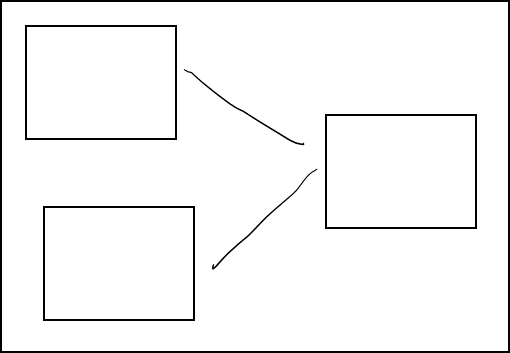
\includegraphics[width=0.5\textwidth]{test}
\end{figure}

\cite{van2019spec}
\cite{Yussupov2019_SystematicMappingStudyFaaS}
\cite{lee2018evaluation}
\cite{aws2020ManagingFunctions}
\\\\
Um provisioned concurrency festzulegen, sollte nachgesehen werden, wie häufig ein Funktion bzw. ein Service aufgerufen wird, und dementsprechend geschaut werden, wie viele Funktionsinstanzen immer vorrätig sein sollten. zudem sollte geprüft werden, wie lange ein Funktionsaufruf von dem Initialen Event bis zu seiner Response braucht, um zu schauen in wie weit dei Preformance durch die Nutzung einer alternativen Programmiersprache gesteigert werden kann. 
Eine weitere Möglichkeit bietet AWS mit Application Auto Scaling welches porvisioned concurrency erweitert ... \textcolor{green}{Target tracking scaling policy, welches provisioned concurrency automatisch napasst, je nach Nutztungsmetrik}
 
\subsection{Auswahl des Service}
\subsection{Abwägung Open-Source und Cloud-Vendor}
Die Abwägung zwischen der Implementation von Function as a Service in der unternehmenseigenen Cloud bzw. Servern oder dem Outsourcen an einen proprietären Cloud-Vendor, sollte wohl überlegt sein, da hiervon in der Folge eine Vielzahl an Möglichkeiten und Restriktionen abhängt. \\\\
Entscheidet man sich für ersteres, also dem Aufbau einer privaten FaaS-Plattform so stehen hierfür, mit IBM Apache Openwhisk, Fission, OpenFaaS oder Kubless, nahezu identisch viele Frameworks zur Verfügung wie bei den öffentlichen Vendoren. \textcolor{blue}{Schaubild CNCF Serverless Landscape ggf. einfügen.} Des Weiteren bietet dieser Weg, abgesehen von der Vielfalt an Frameworks mit wiederum unterschiedlichen Eigenschaften, die Möglichkeit die Größe der Funktionen oder die maximal zulässige Laufzeit eines Containers individuell anzupassen. Dies würde einerseits eine granularer Verrechnung der in Anspruch genommenen Ressourcen der einzelnen Bereiche oder Teams zulassen, zugleich aber auch ein Operations-Team verlangen, welches sich in das jeweilige Framework einarbeitet, die Plattform zu dessen Betrieb aufsetzt und die spätere Wartung dieser übernimmt. \cite{mohanty2018evaluation}.\\\\
Eine Alternative stellen proprietäre Lösungen von öffentlichen Cloud-Vendoren, wie beispielsweise Amazon Web Services (AWS) Lambda, Microsofts Azure Functions, IBM Cloud Functions oder Google Cloud Functions, bei welchen sich von Unternehmensseite aus niemand um die Wartung der Infrastruktur, die Skalierung der Services, die Behandlung von Fehlermeldungen o.ä. kümmern muss. Diese Aufgaben werden in der Folge von dem Plattformbetreiber übernommen. Natürlich sind diese Dinge in erster Linie Aufgabe des Plattformbetreibers, jedoch haben sie unmittelbare Auswirkungen auf das Unternehmen, sollten Probleme beim Skalieren von Funktionen oder dem Monitoring auftreten. Sollte dies der Fall sein, so sind die Entwickler von den bereitgestellten Debugging Möglichkeiten und Monitoring-Lösungen der Plattform abhängig um Probleme schnellstmöglich zu beheben, sollte dies die Plattform nicht tun. Daneben ist ein weiterer Punkt des Vendor Lock-Ins die von Anbieter zu Anbieter variierende Infrastruktur, welche ein einfaches Shiften von Funktionen erheblich erschwert. Zudem sind die Benutzung der Funktionen meist automatisch mit der Inanspruchnahme weiterer Services der Plattform, wie dem Message Queuing oder der Datenspeicherung, gekoppelt. \\\\
Dies hat sowohl Vor- als auch Nachteile. Ist man bei der Einrichtung der privaten FaaS-Cloud auf die unternehmensinternen Ressourcen beschränkt, so bieten die Cloud-Anbieter, neben den Restriktionen des Vendor Lock-Ins, in den meisten Fällen ein großes Ökosystem an weiteren Services, welche sich problemlos an die Funktionen anbinden lassen. Im Folgenden wird daher, auch wenn sich diese Arbeit hauptsächlich auf FaaS beschränkt, das Ökosystem der einzelnen Cloud-Anbieter kurz betrachtet, um einen besseren Überblick über deren zusätzliche Leistungen zu erhalten und eine fundierte Entscheidung treffen zu können.
\subsubsection{Vendoren-Analyse}
Ein weiterer Punkt bei der Migration von Teilen einer besehenden Architektur, in diesem Fall einer Microservice Architektur, ist die von dem Cloud-Vendor zur Verfügung gestellte Möglichkeit der Orchestrierung der Funktionen. Diese entscheidet darüber wie performant die Funktionen parallel ausgeführt werden können und wie groß der Runtime-Overhead der jeweiligen Plattformen dabei ist. Zudem spielt der Preis der hierfür anfällt eine nicht unerhebliche Rolle, da die sequentielle als auch die parallele Ausführung von Funktionen bei mittleren und großen Softwareprojekten häufig auftreten. \\\\
Wie bereits in \textit{Potentiale und Herausforderungen} unter \textit{Statelessness} erwähnt spielt bei der Kopplung von Funktionen die Weitergabe des Anwendungs- bzw. Funktions-\textit{States} und dessen Geschwindigkeit eine wichtige Rolle. Nur durch das richtige Zusammenspiel vieler Funktionen ist es möglich große Anwendungen zu bauen und komplexe Abläufe umzusetzen. Bei der Betrachtung der unterschiedlichen Hosting-Lösungen soll der Fokus auf die beiden am häufigsten genutzen proprietären FaaS-Lösungen \cite{leitner2019mixed}, AWS Lambda mit Amazon Step Functions und Microsoft Azure Functions mit Azure Durable Functions, gelegt werden. Die Seite der Open-Source Lösungen wird von IBM OpenWhisk, mit IBM Composer als Orchestrierungs-Lösung, vertreten.\\\\
\cite{lopez2018comparison} hat diese drei Frameworks genuaer untersucht und in Bezug auf die sequentiell und parallele Planung sowie die Weitergabe des \textit{States} der drei Orchestrierungs-Tool erhebliche Unterschiede feststellen können.  
%The orchestration component defines the sequence of tasks; all executions are automatically triggered, each step is tracked and retried in the case of error \cite{werner2018serverless}. AWS Step Functions Each step of an application is triggered, tracked and even retried when errors occur, assuring that applications execute as expected and in the correct order. To aid debugging and diagnostics, logs are kept for every step of the process. Figure 3 shows this process. An added benefit is that step functions can be created and deployed in code through the definition of a state machine using Amazon’s JSON-based States Language10. \cite{werner2018serverless}. 
Kein garantie, dass der folgende Funktionsaufruf auf die selbe bereits laufende Instanz einer Funktion trifft, welche dann wiederum auch zugriff auf dem im Memory gespeicherten State hat. Es ist daher notwendig, dass der Application-State extern gespeichert wird. Auf diesen sog. "\textit{Shared memory}" müssen in der Folge alle Funktionen drauf zugreifen, wenn Applikations-Daten benötigt werden.
\subsubsection{Tools zur Entwicklungsunterstützung}
IBM Composer, Amazon Step Functions, Azure Durable Functions %These tools allow to define sequences and/or parallel executions of functions and provide strategies to handle execution failures. Finally, many FaaS providers offer metric collection, tracing, and debugging facilities, if only at additional cost. Examples include AWS X-Ray and Google Stackdriver.  \cite{leitner2019mixed}. Beyondprovider-offeredtools, aplethoraofthird-party created tools have emerged. Foremost among them are FaaS deployment tools such as the Serverless framework4, which abstracts from provider-specific aspects of FaaS offerings, allowing to build and deploy provider-independent functions. \cite{leitner2019mixed}
\subsubsection{Cross-Functions in Multi-Cloud Lösung}
\subsection{Auswirkungen auf und Anpassungen der Testumgebungen}
Dies ist teilweise Vendorenspezifisch und bedarf der auseinandersetzung 
\subsection{Konsequenzen für das Monitoring}
\section{Anwendung des Leitfadens}
\subsection{Auswertung der Ergebnisse}
\subsubsection{Beurteilung der Kollaborationsauswirkungen}
\subsubsection{Beurteilung der Stabilität}
\subsubsection{Beurteilung der Skalierbarkeit} 
\subsubsection{Beurteilung des Monitorings}
\subsubsection{Beurteilung der Testmöglichkeiten} 
\subsection{Korrektur und Anpassungen}
\section{Abschließende Betrachtung}
\subsection{Absehbare Entwicklungen}
\cite{al2019systematic} Serverless  immer mehr bekanntheit und mehr Papers etc. ... Später market für funktionen die optimiert sind etc. \cite{shafiei2020serverless}\\
Real time communication tool  \cite{shafiei2020serverless} \\
Real time tracking gps  \cite{shafiei2020serverless} da beide nicht auf dem Application state benötigen/ beruhen  \cite{shafiei2020serverless} \\
\cite{hellerstein2018serverless}
\subsection{Zusammenfassung}
\subsection{Weiterführende Forschung}
Serverless Computing: A Survey of Opportunities, Challenges and Applications store for functions
\cite{shahrad2019architectural}
\newpage
\printbibliography[title={Literaturverzeichnis}]
\end{document}